\documentclass[tikz,border=6mm]{standalone}
\usepackage{amsmath,amssymb}
\usepackage{fontspec}

\usetikzlibrary{positioning,arrows.meta,shapes.geometric,fit,backgrounds,calc}

% Define cohesive professional color palette
\definecolor{navyblue}{RGB}{30, 60, 105}
\definecolor{tealblue}{RGB}{20, 110, 105}
\definecolor{purplecat}{RGB}{95, 45, 120}
\definecolor{ambergold}{RGB}{180, 85, 15}
\definecolor{forestgreen}{RGB}{25, 115, 60}
\definecolor{crimsonred}{RGB}{175, 40, 40}
\definecolor{slategrey}{RGB}{70, 85, 100}

\begin{document}
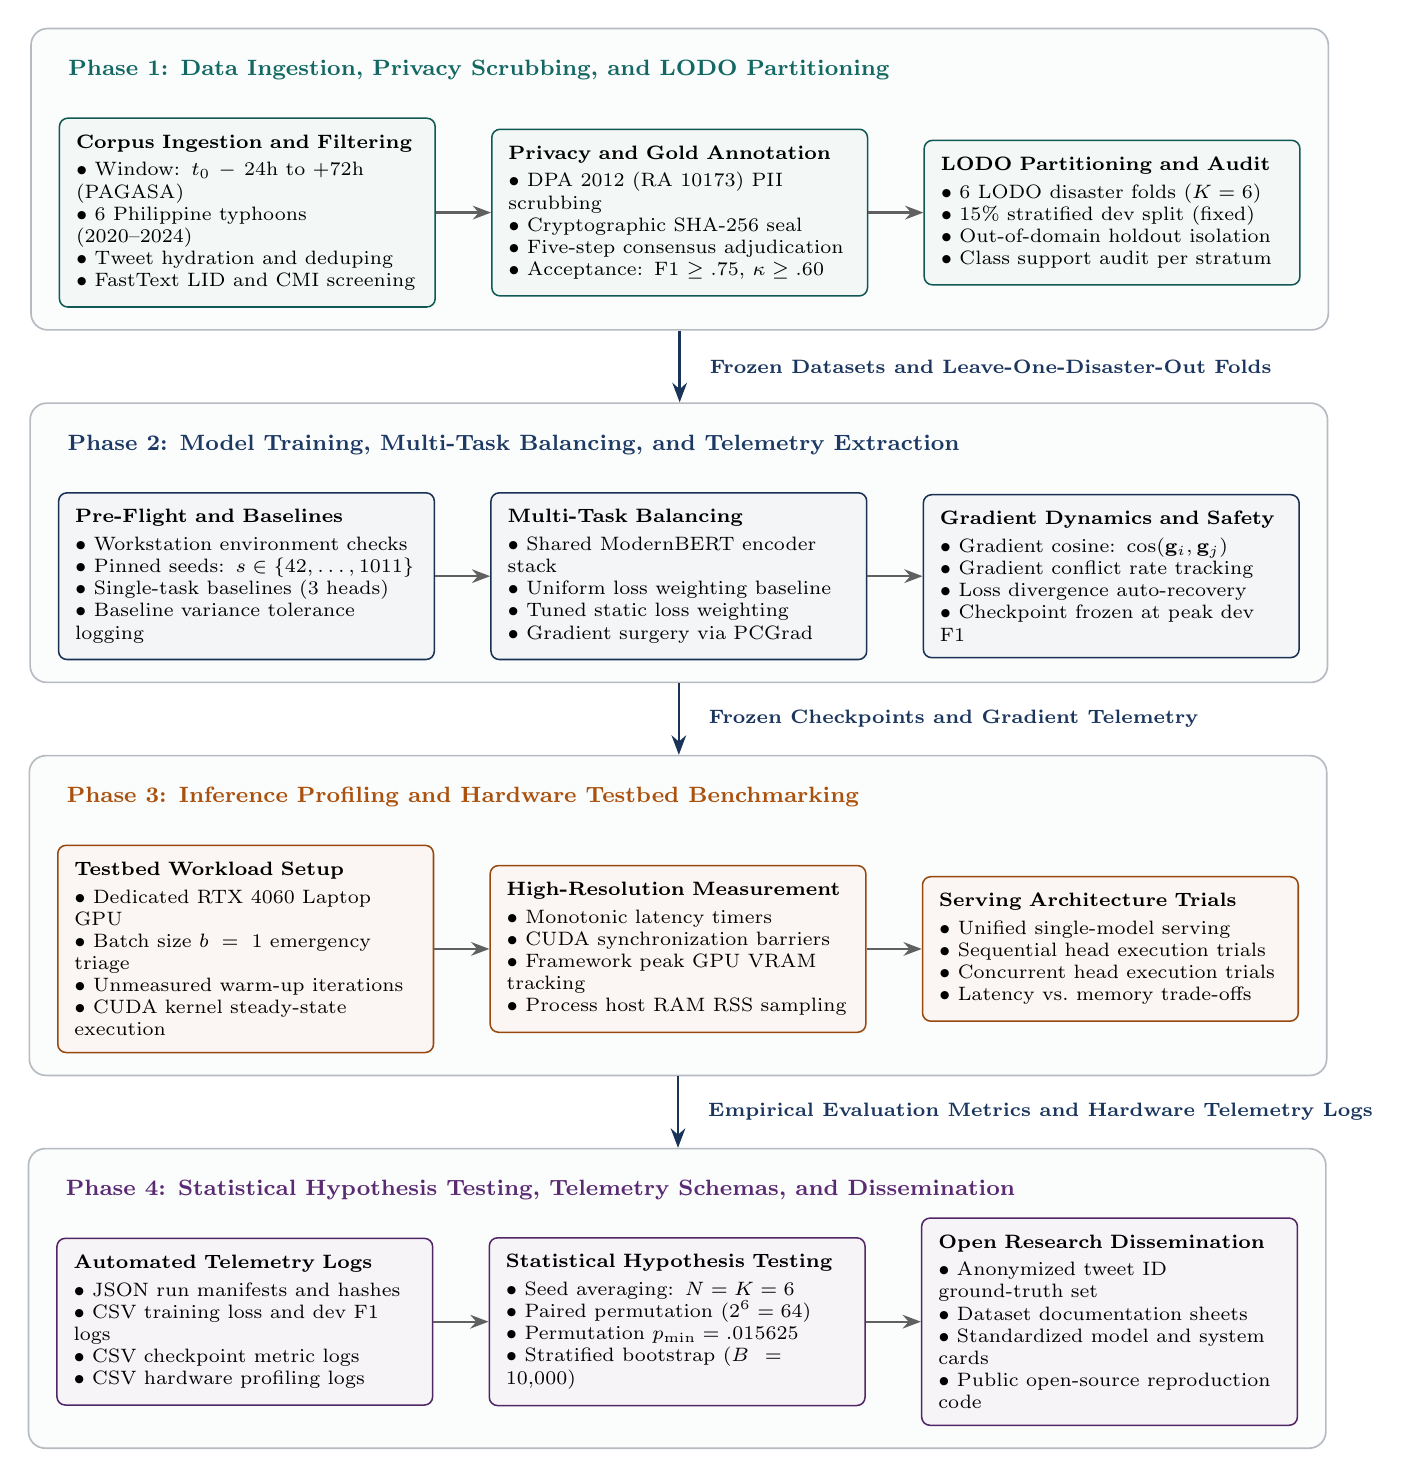
\begin{tikzpicture}[
    font=\small,
    >=Stealth,
    every node/.append style={execute at begin node={\hyphenpenalty=10000\exhyphenpenalty=10000\relax}},
    % Styles
    stagetitle/.style={
        font=\bfseries\footnotesize,
        anchor=west
    },
    procbox/.style={
        draw=gray!50,
        fill=white,
        rounded corners=3pt,
        align=left,
        inner sep=6pt,
        font=\scriptsize,
        line width=0.55pt,
        text width=4.35cm
    },
    flowarrow/.style={
        ->,
        thick,
        draw=gray!75!black
    },
    transarrow/.style={
        ->,
        line width=0.9pt,
        draw=navyblue!85!black
    }
]

    % =========================================================================
    % STAGE 1: DATA INGESTION, PRIVACY, AND PARTITIONING
    % =========================================================================
    \node[stagetitle, text=tealblue!95!black] (title1) at (0, 0) 
        {Phase 1: Data Ingestion, Privacy Scrubbing, and LODO Partitioning};

    \node[procbox, below=0.35cm of title1.south west, anchor=north west, draw=tealblue!80!black, fill=tealblue!5] (p1_1) {
        \textbf{Corpus Ingestion and Filtering}\\[2pt]
        $\bullet$ Window: $t_0 - 24\text{h}$ to $+72\text{h}$ (PAGASA)\\
        $\bullet$ 6 Philippine typhoons (2020--2024)\\
        $\bullet$ Tweet hydration and deduping\\
        $\bullet$ FastText LID and CMI screening
    };

    \node[procbox, right=0.7cm of p1_1, draw=tealblue!80!black, fill=tealblue!5] (p1_2) {
        \textbf{Privacy and Gold Annotation}\\[2pt]
        $\bullet$ DPA 2012 (RA 10173) PII scrubbing\\
        $\bullet$ Cryptographic SHA-256 seal\\
        $\bullet$ Five-step consensus adjudication\\
        $\bullet$ Acceptance: F1 $\ge .75$, $\kappa \ge .60$
    };

    \node[procbox, right=0.7cm of p1_2, draw=tealblue!80!black, fill=tealblue!5] (p1_3) {
        \textbf{LODO Partitioning and Audit}\\[2pt]
        $\bullet$ 6 LODO disaster folds ($K=6$)\\
        $\bullet$ 15\% stratified dev split (fixed)\\
        $\bullet$ Out-of-domain holdout isolation\\
        $\bullet$ Class support audit per stratum
    };

    \draw[flowarrow] (p1_1.east) -- (p1_2.west);
    \draw[flowarrow] (p1_2.east) -- (p1_3.west);

    \begin{scope}[on background layer]
        \node[draw=slategrey!40, fill=slategrey!2, rounded corners=6pt, line width=0.6pt,
              fit=(title1.north west)(p1_1.south west)(p1_3.south east), inner xsep=10pt, inner ysep=8pt] (box1) {};
    \end{scope}

    % =========================================================================
    % STAGE 2: MODEL TRAINING, BALANCING, AND TELEMETRY
    % =========================================================================
    \path (box1.south west) ++(10pt, -1.45cm) node[stagetitle, text=navyblue!95!black, anchor=west] (title2) 
        {Phase 2: Model Training, Multi-Task Balancing, and Telemetry Extraction};

    \node[procbox, below=0.35cm of title2.south west, anchor=north west, draw=navyblue!80!black, fill=navyblue!5] (p2_1) {
        \textbf{Pre-Flight and Baselines}\\[2pt]
        $\bullet$ Workstation environment checks\\
        $\bullet$ Pinned seeds: $s \in \{42, \dots, 1011\}$\\
        $\bullet$ Single-task baselines (3 heads)\\
        $\bullet$ Baseline variance tolerance logging
    };

    \node[procbox, right=0.7cm of p2_1, draw=navyblue!80!black, fill=navyblue!5] (p2_2) {
        \textbf{Multi-Task Balancing}\\[2pt]
        $\bullet$ Shared ModernBERT encoder stack\\
        $\bullet$ Uniform loss weighting baseline\\
        $\bullet$ Tuned static loss weighting\\
        $\bullet$ Gradient surgery via PCGrad
    };

    \node[procbox, right=0.7cm of p2_2, draw=navyblue!80!black, fill=navyblue!5] (p2_3) {
        \textbf{Gradient Dynamics and Safety}\\[2pt]
        $\bullet$ Gradient cosine: $\cos(\mathbf{g}_i, \mathbf{g}_j)$\\
        $\bullet$ Gradient conflict rate tracking\\
        $\bullet$ Loss divergence auto-recovery\\
        $\bullet$ Checkpoint frozen at peak dev F1
    };

    \draw[flowarrow] (p2_1.east) -- (p2_2.west);
    \draw[flowarrow] (p2_2.east) -- (p2_3.west);

    \begin{scope}[on background layer]
        \node[draw=slategrey!40, fill=slategrey!2, rounded corners=6pt, line width=0.6pt,
              fit=(title2.north west)(p2_1.south west)(p2_3.south east), inner xsep=10pt, inner ysep=8pt] (box2) {};
    \end{scope}

    % =========================================================================
    % STAGE 3: INFERENCE PROFILING AND HARDWARE BENCHMARKING
    % =========================================================================
    \path (box2.south west) ++(10pt, -1.45cm) node[stagetitle, text=ambergold!95!black, anchor=west] (title3) 
        {Phase 3: Inference Profiling and Hardware Testbed Benchmarking};

    \node[procbox, below=0.35cm of title3.south west, anchor=north west, draw=ambergold!85!black, fill=ambergold!5] (p3_1) {
        \textbf{Testbed Workload Setup}\\[2pt]
        $\bullet$ Dedicated RTX 4060 Laptop GPU\\
        $\bullet$ Batch size $b=1$ emergency triage\\
        $\bullet$ Unmeasured warm-up iterations\\
        $\bullet$ CUDA kernel steady-state execution
    };

    \node[procbox, right=0.7cm of p3_1, draw=ambergold!85!black, fill=ambergold!5] (p3_2) {
        \textbf{High-Resolution Measurement}\\[2pt]
        $\bullet$ Monotonic latency timers\\
        $\bullet$ CUDA synchronization barriers\\
        $\bullet$ Framework peak GPU VRAM tracking\\
        $\bullet$ Process host RAM RSS sampling
    };

    \node[procbox, right=0.7cm of p3_2, draw=ambergold!85!black, fill=ambergold!5] (p3_3) {
        \textbf{Serving Architecture Trials}\\[2pt]
        $\bullet$ Unified single-model serving\\
        $\bullet$ Sequential head execution trials\\
        $\bullet$ Concurrent head execution trials\\
        $\bullet$ Latency vs.\ memory trade-offs
    };

    \draw[flowarrow] (p3_1.east) -- (p3_2.west);
    \draw[flowarrow] (p3_2.east) -- (p3_3.west);

    \begin{scope}[on background layer]
        \node[draw=slategrey!40, fill=slategrey!2, rounded corners=6pt, line width=0.6pt,
              fit=(title3.north west)(p3_1.south west)(p3_3.south east), inner xsep=10pt, inner ysep=8pt] (box3) {};
    \end{scope}

    % =========================================================================
    % STAGE 4: STATISTICAL INFERENCE AND DISSEMINATION
    % =========================================================================
    \path (box3.south west) ++(10pt, -1.45cm) node[stagetitle, text=purplecat!95!black, anchor=west] (title4) 
        {Phase 4: Statistical Hypothesis Testing, Telemetry Schemas, and Dissemination};

    \node[procbox, below=0.35cm of title4.south west, anchor=north west, draw=purplecat!85!black, fill=purplecat!5] (p4_1) {
        \textbf{Automated Telemetry Logs}\\[2pt]
        $\bullet$ JSON run manifests and hashes\\
        $\bullet$ CSV training loss and dev F1 logs\\
        $\bullet$ CSV checkpoint metric logs\\
        $\bullet$ CSV hardware profiling logs
    };

    \node[procbox, right=0.7cm of p4_1, draw=purplecat!85!black, fill=purplecat!5] (p4_2) {
        \textbf{Statistical Hypothesis Testing}\\[2pt]
        $\bullet$ Seed averaging: $N=K=6$\\
        $\bullet$ Paired permutation ($2^6 = 64$)\\
        $\bullet$ Permutation $p_{\min} = .015625$\\
        $\bullet$ Stratified bootstrap ($B = \text{10,000}$)
    };

    \node[procbox, right=0.7cm of p4_2, draw=purplecat!85!black, fill=purplecat!5] (p4_3) {
        \textbf{Open Research Dissemination}\\[2pt]
        $\bullet$ Anonymized tweet ID ground-truth set\\
        $\bullet$ Dataset documentation sheets\\
        $\bullet$ Standardized model and system cards\\
        $\bullet$ Public open-source reproduction code
    };

    \draw[flowarrow] (p4_1.east) -- (p4_2.west);
    \draw[flowarrow] (p4_2.east) -- (p4_3.west);

    \begin{scope}[on background layer]
        \node[draw=slategrey!40, fill=slategrey!2, rounded corners=6pt, line width=0.6pt,
              fit=(title4.north west)(p4_1.south west)(p4_3.south east), inner xsep=10pt, inner ysep=8pt] (box4) {};
    \end{scope}

    % =========================================================================
    % MAJOR INTER-STAGE TRANSITION ARROWS
    % Strictly vertical plumb-lines connecting container boundaries
    % =========================================================================
    \draw[transarrow] (p1_2.south |- box1.south) -- (p1_2.south |- box2.north)
        node[midway, right=0.25cm, font=\scriptsize\bfseries, text=navyblue!90!black] 
        {Frozen Datasets and Leave-One-Disaster-Out Folds};

    \draw[transarrow] (p2_2.south |- box2.south) -- (p2_2.south |- box3.north)
        node[midway, right=0.25cm, font=\scriptsize\bfseries, text=navyblue!90!black] 
        {Frozen Checkpoints and Gradient Telemetry};

    \draw[transarrow] (p3_2.south |- box3.south) -- (p3_2.south |- box4.north)
        node[midway, right=0.25cm, font=\scriptsize\bfseries, text=navyblue!90!black] 
        {Empirical Evaluation Metrics and Hardware Telemetry Logs};

\end{tikzpicture}
\end{document}
